\chapter{BLE positioning in practice}
\label{chap:architecture}

\section{RSS based positioning}
\label{sec:architecture-rss-based-positioning}
\citet{bahl2000radar} laid the foundation for positioning using \wifi signals.
The basis is a fingerprint database, containing fingerprints (the RSS, or RSS distribution, for each access point) for a large number of locations.
This database can either be filled empirically, surveying the RSS at each location; or calculated, where the RSS at each location is estimated using the positions of the access points and a radio propagation model for the environment.
They show that empirically filling the database leads to better results, however it may take much longer since a manual survey of each location is needed.

To do positioning, a measurement of the RSS of each access point at an unknown location is made, and each fingerprint in the database is compared to this measurement in order to find one or multiple close matches.
The method mostly used to find a match is (a variant of) k-nearest-neighbour.
The method works in three steps.

Firstly the set of measured RSS are transformed into values needed for step two.
\citet{bahl2000radar} described that the mean, standard deviation and median of multiple measurements at a single location were calculated, but only used the mean in the rest of the paper.

Secondly the values from the fingerprints are compared to the values found while positioning, and a distance between the two sets is determined, by a distance-function $L$.
The usual choice for the distance-function (and hence the name) is to calculate the distance in signal-space, where each signal-source is a dimension.
\citet{li2005method} described a generalised distance function (\equationref{architecture}{distance}).
\begin{equation}
    L_q = \left(\sum_{i=1}^{n}|p_i-s_i|^q\right)^{\frac{1}{q}}
    \label{eq:architecture-distance}
\end{equation}
Here $n$ is the number of signal-sources, $p_i$ the measured RSS for a source during positioning, and $s_i$ the surveyed RSS at the point to which the distance is to be calculated; different $q$ lead to different distance functions with $L_1$ being the Manhattan distance, and $L_2$ the Euclidean distance.
There seems to be no clear consensus on which $q$ gives the best result, with \citet{shin2012enhanced} using $L_1$, \citet{bahl2000radar} using $L_2$, only saying that alternatives (possibly also of another form) were briefly experimented with, and \citet{li2005method} using $L_1$, while noting that the difference with other $q$ values is not significant.
Most methods use the $L_q$ function with the $s_i$/$p_i$ in dB, \citet{li2005method} explores whether these values should alternatively use the power $P$, $1/P$, $1/P^2$ or $1/P^4$, concluding that dB works the best, but $1/P^2$ and $1/P^4$ also give good results.
Another interesting candidate is the Mahalanobis distance, use of which is explored and found to be superior by \citep{kaemarungsi2005efficient}.

Finally the calculated distances are being used to map to a position.
\citet{bahl2000radar} uses both a 1-nearest-neighbour and a k-nearest-neighbour approach, showing that the second works better.
\citet{li2005method} uses a weighted-k-nearest-neighbour approach, where the nearest neighbours are being weighted by the result of the distance-calculation, and \citet{shin2012enhanced} introduced using a dynamic value for the number of neighbours $k$ to further improve the result.

\citet{pandya2003indoor} compares nearest-neighbour to other positioning methods based on RSS, and finds nearest-neighbour to work well in most cases (among which Bluetooth Classic).
Unsurprisingly, methods from the domain of machine learning have been examined as well to do positioning, such as Gaussian Process Latent Variable Models \citep[ferris2007wifi] or Neural Networks \citep[battiti2002location].

Of these methods, the one used by \citet{bahl2000radar} is used in this report to compare against; both because the method is simple to understand and implement while giving good results, and because many other authors used this method as a base to compare against.

\section{Experiment}
\label{sec:architecture-experiment}
\fig{\gnuplot{architecture}{room}{Test bed: room SW02 in the Computer Laboratory of the University of Cambridge.}}
Room SW02 in the Computer Laboratory of the University of Cambridge is the test bed for this experiment.
The room consists of a square 12 by 12 meter main area, with several coves.
The room contains four decagonal-shaped tables with computers on them and chairs around them, as well as some other furniture.
Twenty BLE beacons were used, ten on the walls of the room, eight on the tables, one in the middle and one placed a couple of meters outside the room (\figureref{architecture}{room}).
The beacon positions were chosen such that all areas would receive BLE signals, but no specific action was taken to find optimal positions.
Each beacon broadcasts a single advertising packet, a unique \bid, on all three channels, with a rate of 10Hz.
All measurements were done on a 60 by 60 cm grid, since this is the size of the floor tiles and this allowed for easy reference.

\fig{
    \centering{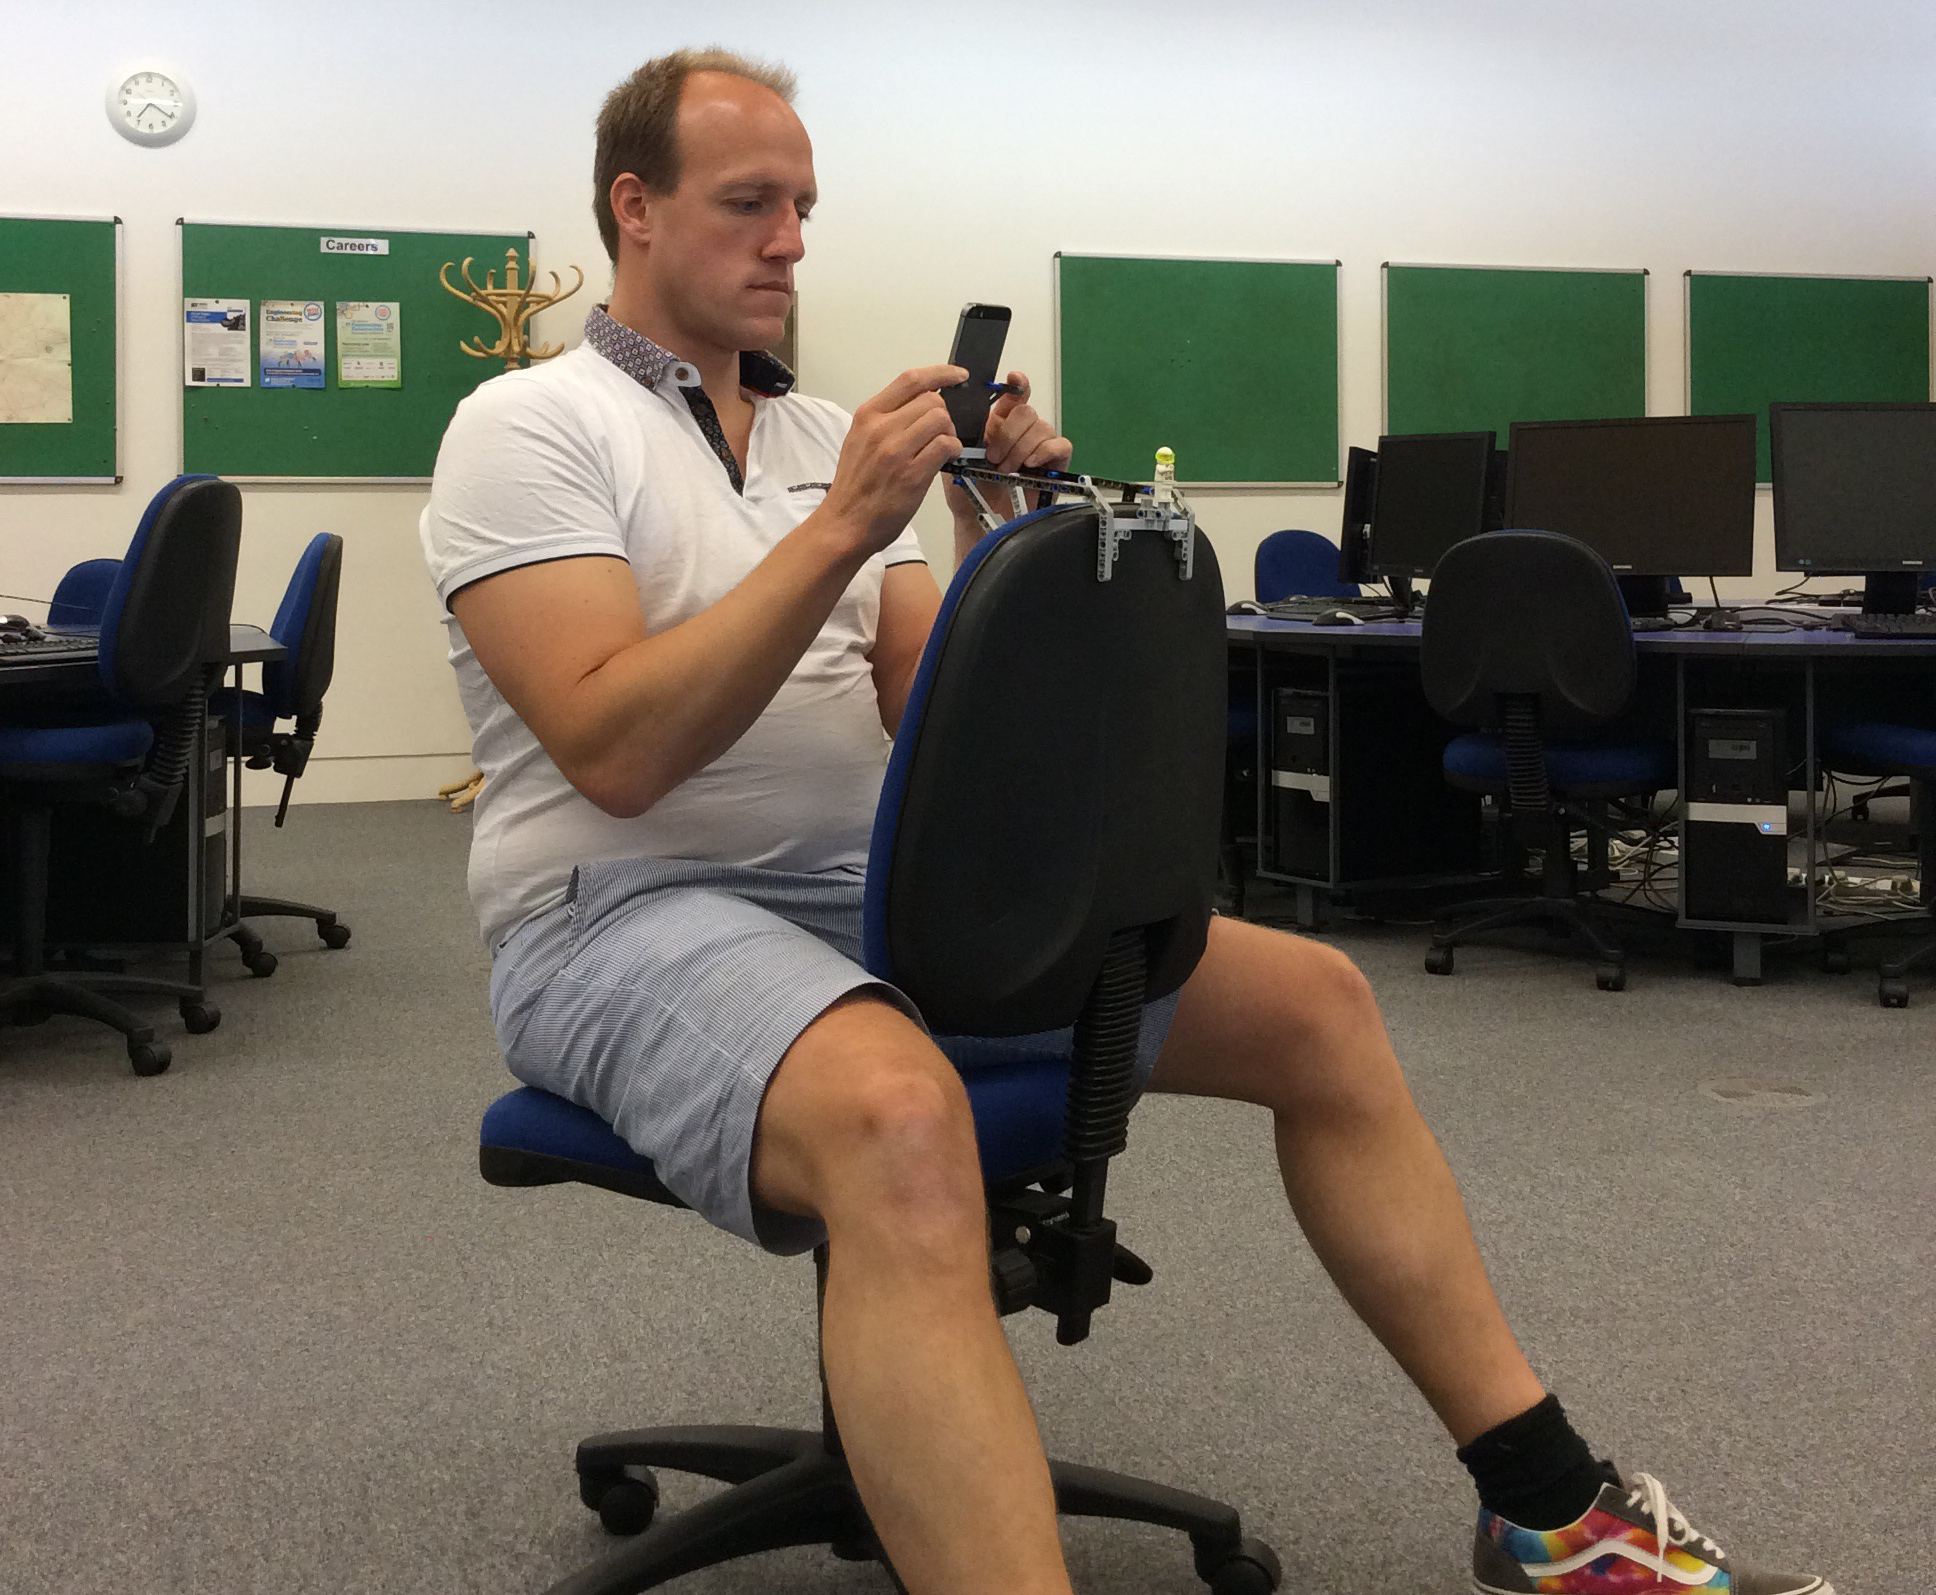
\includegraphics[width=0.7\textwidth]{images/survey}}
    \caption{Device used for surveying.}
    \label{fig:architecture-survey-device}
}

During the surveying phase, each accessible point on the grid is surveyed, by slowly moving the \device along a circle with a radius of 15 cm centred on the grid point, the back of the phone facing outwards, with a human body on the opposite side of the circle, facing the screen; the normal position for a user using the \device.
To accomplish this consistently, I adjusted the office-chair set-up of \sectionref{rss}{rot}, such that the \device now rotates along a circle instead of its axis (\figureref{architecture}{survey-device}).
For each advertisement packet received, the \bid, advertising channel, RSS and the current heading as reported by the \device's compass, is saved.
Complete 360\tdegree survey took between 3.5 and 15 seconds for each of the 226 accessible points, with a mean of 9 seconds per point.
On average 903 advertising packets were captured per point, meaning there was around 45\% packet loss.

During the positioning phase, I went to each grid point, standing naturally while holding the \device still over the grid point for two seconds.
In total 670 positionings measurements were taken at 226 locations.

During surveying each beacon was observed at least once at each location.
During positioning, this was not the case; this may have been because the \device was not moving, not rotating, and the listening interval was shorter.

In addition the $x$, $y$ and $z$ coordinates for each beacon were determined, and the maximum RSS on 1 meter distance.

The data gathered from this experiment allows me to compare six different positioning algorithms, and simulate how they perform under different circumstances.

\section{Positioning methods}

All positioning in this report is being done through the weighted k-nearest-neighbour algorithm.
Provided a set of distances for a single measurement to each surveyed point, ordered by distance, the average of the points belonging to the first $k$ distances is calculated, weighted by $\frac{1}{distance+\epsilon}$, to avoid division by 0; an $\epsilon$ of 0.01 was empirically found to work well.
The difference between the compared algorithms, is in how the distances are calculated, the first two steps of the nearest-neighbour algorithm as described in \sectionref{architecture}{rss-based-positioning}.
All experiments are run with $k = 5$; this value was empirically found to work well.

In the positioning algorithms below, the first step is always (except for ``random'') taking either the mean or the maximum RSS measured at a location.
To deal with cases when a particular beacon was not observed, that beacon is treated as having been received with an RSS of -105dB; this is 2dB lower than the lowest RSS reported for an actual packet during the experiment, and seems reasonable, since if there had been a packet with signal strength -105dB, the \device would not have noticed it.

\subsection{Random}
As a reference, the random method returns random distances for each fingerprint, after which the k-nearest-neighbours method is used to calculate a position.

\subsection{Signal Space Distance (SSD)}
The method described in \citet{bahl2000radar}, using dB for the RSS, and the $L_2$ distance function (\equationref{architecture}{distance}).
As in \citet{bahl2000radar}, the mean RSS over all received packets is used both in the surveying and the positioning data.
Only one fingerprint per position is taken, unlike \citet{bahl2000radar}, who created four fingerprints in four different directions.

\subsection{Signal Space Distance with Orientation (SSD-O)}
\label{sec:architecture-ssd-o}
In \sectionref{rss}{rot} I showed that the direction of measurement has a huge influence on the RSS.
\citet{bahl2000radar} recognised this in \wifi, and surveyed in four directions; during positioning however they had no way to determine the orientation, and all four directions were considered equally during positioning.
\citet{king2006compass} considered how knowledge of the orientation improves positioning.
They surveyed in eight directions, and considered different ways of combining these into ad-hoc fingerprints during positioning.

I consider a variant of King's method, using the Signal Space Distance, but taking orientation into consideration: SSD-O.
Unlike the \wifi surveying used by \citet{bahl2000radar} and \citet{king2006compass}, I survey continuously while turning 360\tdegree.
For each packet received, the heading as reported by the \device's compass is stored in the database, with the \bid and the RSS.
While positioning, the \device is expected to not be rotating much; the average heading $h_p$ of the device is used to build an ad-hoc fingerprinting database.
This database is built using the mean RSS, where at each location, for each beacon, only those packets are considered that were received during surveying with a heading $h_s$ where $h_p - \alpha < h_s < h_p + \alpha$.
A value of 60\tdegree for $\alpha$ was found to work best (see \sectionref{architecture}{measurements}).
In order to not have to calculate the ad-hoc fingerprint database for each positioning, the experiment was run with 360 pre-calculated fingerprint databases, one per 1\tdegree, where for each positioning the closest database is used.
For example, if the average heading during positioning is 34.6\tdegree, the pre-calculated database at 35\tdegree will be used, which is built using all surveying packets that were received between 335\tdegree and 95\tdegree.

It should be noted that this method is dependent on the accuracy of the built-in compass.
During surveying and positioning I kept an eye on the compass reading, and noticed nothing absurd, however no further effort was made to check how accurate the compass is.
In \sectionref{architecture}{measurements-ssd-o}, I explore the influence that a potential compass-error has on this method.

\subsection{\BRP (\aBRP)}
\label{sec:architecture-brp}
\begin{figure}[p]
    \begin{subfigure}[b]{0.5\textwidth}
        \gnuplotscale{architecture}{rss-cloud-2.0s}{2.0s}{0.55}
    \end{subfigure}
    \begin{subfigure}[b]{0.5\textwidth}
        \gnuplotscale{architecture}{rss-cloud-1.0s}{1.0s}{0.55}
    \end{subfigure}
    \begin{subfigure}[b]{0.5\textwidth}
        \gnuplotscale{architecture}{rss-cloud-0.5s}{0.5s}{0.55}
    \end{subfigure}
    \begin{subfigure}[b]{0.5\textwidth}
        \gnuplotscale{architecture}{rss-cloud-0.2s}{0.2s}{0.55}
    \end{subfigure}
    \caption{Relation between the maximum RSS per beacon measured in a spot during surveying and positioning, for different listening times. If a beacon is not observed, it is assigned an RSS of -105dB.}
    \label{fig:architecture-rss-cloud}
\end{figure}

I introduce \BRP to do positioning with \BLE, taking into account some of the radio propagation properties of BLE that were described in \chapterref{rss}. 
Most notably, the method recognises that some beacons may be temporarily blacked-out; they may be received at much lower RSS or not at all due to \mpi, orientation, body shadowing or packet loss.

\aBRP uses the same k-nearest-neighbour approach as the previous methods, however since it does not calculate distance between a fingerprint and the measurement in a multi-dimensional signal space, it intuitively makes more sense to talk about a \define{penalty function} in this context.
The function gives penalty points for each way in which a fingerprint does not agree with a positioning measurement.
This syntactic difference does not change its semantics however: penalties are calculated for each fingerprint in the database, and the ones with the lowest penalties are selected to be averaged.

\BRP recognises that, once during surveying the maximum RSS $s_i$ in an area has been determined for a certain beacon, it is unlikely that during positioning a much higher RSS $p_i$ will be measured at that point.
This means that $p_i \gg s_i$ should result in a large penalty.
On the other hand, having measured a much lower RSS may be the result of \mpi, antenna orientation, body shadowing, or packet loss, and is not a strong indicator that a particular position should be discarded; hence $p_i \ll s_i$ should not carry a large penalty.
Obviously the lowest penalty is given if $p_i \approx s_i$.
By adding the individual penalties given per beacon together, the full penalty for a fingerprint is obtained.

\Figureref{architecture}{rss-cloud} shows how $s_i$ relates to the $p_i$ on the same location.
The figures show that $p_i$ is on average a couple of dB lower than $s_i$; it shows that my assumption that $p_i$ is not much higher than $s_i$ is correct, and shows that there are many situations where $p_i \ll s_i$.
Shorter listening intervals lead to a higher difference between $s_i$ and $p_i$, which is to be expected since $p_i$ is the maximum for all packets, and a shorter listening period will give a smaller maximum on average.
The points on the left side, where $p_i$ = -105dB indicate those situations when a certain beacon was not observed during the listening interval.

\fig{\gnuplot{architecture}{penalty}{Penalty function for \aBRP, as compared to SSD}}

The following penalty function was empirically found to work well.
It is based on $d_i$, which is the difference between $p_i$ and $s_i$.
A positive $d_i$ indicates that the measured RSS during positioning is larger than the RSS surveyed for a candidate location.
\begin{equation}
    L = \begin{cases}
        |d_i| \times 100000 +3.042  & \text{if } d_i > 3dB \\
        |d_i| +0.042                & \text{if } 0dB < d_i \leq 3dB \\
        |d_i+4.2| \times 0.01       & \text{if } -10dB < d_i \leq 0dB \\
        |d_i| \times 0.125          & \text{if } d_i \leq -10dB 
    \end{cases}
    \label{eq:architecture-BRP-punishment}
\end{equation}
This penalty function is shown in \figureref{architecture}{penalty} and compared to the (scaled) Euclidean distance function.

The function can be understood by realising that for $d_i > 0dB$, large and very large penalties are given (top two lines).
For $d_i < -10$dB, penalties start with a large offset, but increase only slowly as $d_i$ decreases.
The part in between has very low penalties with a minimum of 0 at $d_i = -4.2$.
This is the average $d_i$ for the 2 second listening interval.

The function has been optimised for performance on the 2 second listening interval, however while keeping performance in other situations in mind as well.
Considering the changes in $d_i$ distribution for different listening intervals, as shown in \figureref{architecture}{rss-cloud}, optimising for other listening intervals will probably lead to other parameters.

\subsection{\BRP with Orientation (\aBRP-O)}
Taking orientation into account in \aBRP, in the same way that SSD-O does for SSD, is an obvious extension.
It should be noted however that \aBRP is specifically designed to have a certain resistance to signal drops, including those from orientation.

In SSD-O, $\alpha$ = 60\tdegree was found to work best; in \aBRP-O $\alpha$ = 90\tdegree works best.

\subsection{\BRP with Radio Propagation Model (\aBRP-RPM)}
Whereas \aBRP uses a surveyed database of fingerprints, \aBRP-RPM estimates the maximum RSS on a specific location using a radio propagation model.
\citet{bahl2000radar} describe a radio propagation model used for \wifi signals, which uses the layout of the building, and a Wall Attenuation Factor to estimate RSS at different locations.
Such a model does not work well for \aBRP however, since \aBRP expects the fingerprints to be the maximum receivable RSS in that area, and the model in \citet{bahl2000radar} tries to have a low average error.
Instead I use a simplified model for maximum expected RSS at a position.

\begin{equation}
    R(x) = R_0 - 10 \times \, ^{10}\log(x^2) = R_0 - 20 \times \, ^{10}\log(x)
\end{equation}

By measuring the RSS at one meter for each beacon (if all beacons are similar, this only has to be measured for one beacon), this formula can be used to estimate the maximum RSS at any location.

\section{Measurements}
\label{sec:architecture-measurements}
\begin{figure}[p]
    \begin{subfigure}[b]{0.5\textwidth}
        \gnuplotscale{architecture}{heatmap-f-mean}{mean (SSD)}{0.55}
    \end{subfigure}
    \begin{subfigure}[b]{0.5\textwidth}
        \gnuplotscale{architecture}{heatmap-f-ssd-o-0}{mean, direction north (SSD-O)}{0.55}
    \end{subfigure}
    \begin{subfigure}[b]{0.5\textwidth}
        \gnuplotscale{architecture}{heatmap-f-max}{maximum (\aBRP)}{0.55}
    \end{subfigure}
    \begin{subfigure}[b]{0.5\textwidth}
        \gnuplotscale{architecture}{heatmap-f-brp-o-0}{maximum, direction north (\aBRP-O)}{0.55}
    \end{subfigure}
    \caption{Each method uses its own fingerprint database; shown the RSS of the central beacon in each database}
    \label{fig:architecture-heatmaps}
\end{figure}

\Figureref{architecture}{heatmaps} shows the RSS for a single beacon in the different fingerprint databases.
The RSS looks as expected; RSS generally decreases with distance to the beacon.
The SSD-O fingerprint has slightly higher averages than the SSD south of the beacon, and slightly lower north of the beacon, because of body shadowing.
The maximum RSS (as shown in (c)) is about 10dB higher than the mean, with \aBRP-O showing the same slight directional properties.

\fig{\gnuplot{architecture}{results}{Errors for the six positioning methods and two combined methods}}

\subsection{Random}
Using a (deterministic) random distance function gives a mean error of around 6 meters, something that was expected considering that the k-nearest-neighbour algorithm will have a tendency to choose positions in the middle of the room as it averages $k$ positions.
Obviously this would grow with the size of the test bed; it does give a lower bound for positioning.

\subsection{Signal Space Distance}
\fig{\gnuplot{architecture}{positioning-errors-SSD}{Positioning errors using SSD, colour indicates average error, arrows indicate the direction where the algorithm calculated the \device to be.}}
SSD gives a median error of 1.08 meter, and counts as the positioning function the other ones are evaluated against.
\Figureref{architecture}{positioning-errors-SSD} shows that some areas in the room have a larger mean error than other areas, while the arrows show no obvious direction in which the errors lie.

In general positioning seems to be more accurate close to the walls; one explanation may be that orientation and \mpi influence the reception less close to the wall than in the middle of the room, because reflection off the wall compensates for that.
I have been unable to find evidence for this however.

\subsection{Signal Space Distance with Orientation}
\label{sec:architecture-measurements-ssd-o}
\fig{\gnuplot{architecture}{ssd-o-parameter-effect}{Positioning errors using SSD-O, for different values for $\alpha$, and different number of databases.}}
\Figureref{architecture}{results} shows that using the internal compass to take orientation into account can improve positioning performance; in the experiment the error was between 10\%-20\% lower for SSD-O versus SSD, and even more for the upper percentiles.

The average heading stored for all packets received at a single positioning is calculated (since the \device is held still during positioning, all spread in heading is due to noise), and a pre-calculated fingerprint database is used which only considered all surveyed packages in an angle of $\alpha$ = 60\tdegree to the left and right of this heading.
In total, 360 SSD-O databases were pre-calculated, one per 1\tdegree.

\Figureref{architecture}{ssd-o-parameter-effect} shows how the median error changes, if $\alpha$ and the number of databases are adjusted.
It shows that an $\alpha$ of 45\tdegree or 60\tdegree performs best, however all databases between 30\tdegree and 90\tdegree perform close to one another.
Intuitively one may expect databases with smaller $\alpha$ to perform better, however each location was only surveyed for 9 seconds on average, meaning that each 30\tdegree part was only surveyed during 0.75 seconds, or 7.5 beacon intervals, on average.
\Sectionref{rss}{packet-loss} showed that in 7.5 beacon intervals, there is still a reasonable chance that a certain beacon was not observed; and even if all beacons were observed, multiple packets are preferred to come to a good mean.
Indeed 1\% of values in the SSD-O fingerprint database for $\alpha$ = 15 is -105dB.

A single fingerprint database is in the order of 20 bytes per $m^2$ (see \sectionref{architecture}{database}); if we need 360 databases (one per \tdegree), this increases to 7 kilobyte.
\Figureref{architecture}{ssd-o-parameter-effect} shows that more databases generally improve performance, however especially above 36 the change is small, and even with just 3 or 4 databases, performance is better than in the SSD case (the 180\tdegree line).
How many databases should be pre-calculated depends on the application and the amount of storage space available for the databases.

\fig{\gnuplot{architecture}{positioning-compass-error-ssd}{Influence of compass error on SSD-O.}}
SSD-O uses the device's compass to determine orientation.
During surveying and positioning no obvious errors in the orientation reported by the \device's compass were observed, however the compass accuracy was not measured.
In other environment the \device's compass was seen to give errors that were off by 90\tdegree, therefore it is interesting to look at what happens when the compass device gives wrong readings.
For \figureref{architecture}{positioning-compass-error-ssd} the heading readings during the positioning were offset by different values.
The figure shows that SSD-O outperforms SSD with errors of less than 30-60\tdegree.

\subsection{\BRP}
\Figureref{architecture}{results} shows that \aBRP slightly outperforms SSD, however not by much, and worse than SSD-O.
It is still interesting because it gives an alternative positioning method, based on the radio properties of BLE, and because it is more resilient against unobserved beacons, either because of a shorter listening period (\sectionref{architecture}{short-walk}) or because of other reasons (\sectionref{architecture}{dying-beacons}).

It is also of interest that \aBRP and SSD have errors in different locations; a combination of the two could be used to further improve positioning, although the way in which to make this combination needs further research.
As \figureref{architecture}{results} shows, taking the average of the locations returned by SSD and \aBRP (labelled SSD+\aBRP), already results in a positioning method that is better than either one.

\subsection{\BRP with Orientation}
\fig{\gnuplot{architecture}{brp-o-parameter-effect}{Positioning errors using \aBRP-O, for different values for $\alpha$, and different number of databases.}}
As expected, \aBRP-O does not give the same performance benefits over \aBRP as SSD-O has over SSD.
It has the same median performance as \aBRP, it does however have a lower mean (1.19m vs 1.25m) and 75th percentile (1.58m vs 1.67m).
It should be noted however that the \aBRP penalty function was optimised for the \aBRP situation, and different parameters are needed for the \aBRP-O function.
In \sectionref{architecture}{short-walk} I show that \aBRP-O does outperform all other methods on shorter listening intervals.

I change the same parameters for \aBRP-O as I did for SSD-O.
A larger $\alpha$ gives a smaller error; it is possible that choosing different parameters for the penalty function results in different optimal $\alpha$.
As \figureref{architecture}{brp-o-parameter-effect} shows, reduction of the number of databases to 36 or even 12 or 6 can be done without sacrificing much accuracy; some $\alpha$ lines even seem to increase with fewer databases, I expect this to be by chance though.

\Figureref{architecture}{results} shows that, although \aBRP-O performs worse than SSD-O, taking the average of the locations of both (labelled SSD-O+\aBRP-O), results in better performance, especially for those locations with a larger error.

\subsection{\BRP-Radio Propagation Model}
\label{sec:architecture-measurements-brp-rpm}
\aBRP-RPM performs twice as bad as SSD and \aBRP, however the main advantage is that no surveying has to be done, and the database is extremely small; it only needs to contain information on each beacon's location and transmit power.
Efficiently encoded this information is 12 bytes\footnote{
    Assume we want a world-wide coordinate system with a resolution in the cm-range.
    Earth's surface area is 510,072,000 $km^2$; any usable coordinate is between -10km and +200km in height, giving 107,115,120,000 $km^3$, or $10^{26} cm^3$ to address -- any errors due to the earth not being flat fall within error margins.
    11 bytes covers $3\times 10^{26}$ addresses.
    The RSS value is only 1 byte, hence 12 byte is enough.
}, so a beacon could include this information in its advertising packet, completely removing the need for a database.

\section{Change parameters}
During this section I look at the performance of the different methods when certain parameters in the system are changed.
Throughout the section the median error is used for the performance; I have found this to be a good indicator for the performance of the whole system.

In sections \ref{sec:architecture-number-beacons}, \ref{sec:architecture-dying-beacons} and \ref{sec:architecture-number-surveyed-points} I ``randomly'' remove beacons and surveying points.
In these cases the results are gotten by doing 100 iterations, removing the beacons and points in a different order each time.
The order in which the beacons and points are removed is determined by sorting md5-hashes of the \bid/point coordinates and the iteration number, resulting in a deterministic pseudo-random order.
The median error plotted is the average of the median errors of the 100 iterations.


\subsection{Number of beacons}
\label{sec:architecture-number-beacons}
\fig{\gnuplot{architecture}{beaconcount}{Effect of the number of beacons}}
Every beacon added improves positioning, but results in diminishing return.
The test bed contained 20 beacons, about 0.1 per $m^2$.
\Figureref{architecture}{beaconcount} shows all methods having gradually increasing errors when fewer beacons are used.
This effect is slightly smaller in the \aBRP-based methods, and they outperform SSD-O for a small number of beacons.


\subsection{Unobserved beacons}
\label{sec:architecture-dying-beacons}
\fig{\gnuplot{architecture}{livebeaconcount}{Effect of unobserved beacons}}
In the previous section, I considered what happens if there are fewer beacons, both during surveying and positioning.
In this section I explore what happens if the beacons were seen during surveying (hence are present in the fingerprint database), but not during positioning.
This may be because a beacon was switched off, the battery died or the beacon was purposefully removed in a denial-of-service attack.
Since \wifi access points are plugged in to mains, and they are usually in locations not easily accessible to attackers, they are less likely to suffer from the latter two failures than BLE beacons.

Another reason that a beacon may be unobserved is that all packets from the beacon during the listening interval were lost.
\Sectionref{rss}{busyroom} shows that there is a lot of packet loss, and beacons may not be observed, even after several beaconing intervals.
This specific situation is investigated more in \sectionref{architecture}{short-walk}, where the listening intervals are shortened.

If no packets have been received from a beacon during either surveying or positioning, the algorithms used set its average and maximum RSS -105dB.

\Figureref{architecture}{livebeaconcount} shows that the both SSD based methods are very sensitive to unobserved beacons.
A single unobserved beacon almost doubles the mean error for both methods.
The \aBRP methods however are designed to resist blacked-out beacons, and only show gradually increasing errors in a situation where beacons are not observed.
Even with a single unobserved beacon, \aBRP outperforms SSD-O and SSD by having a 35\% and 42\% smaller median error.

\subsection{Positioning listening length}
\label{sec:architecture-short-walk}
\fig{\gnuplot{architecture}{unobserved}{Percentage of positionings with unobserved beacons}}
\fig{\gnuplot{architecture}{short-walk}{Effect of positioning listening interval on median error}}
As described in \sectionref{architecture}{experiment}, positioning was done by listening at a single location for 2 seconds.
On average, 197 packets were received during one positioning, meaning a 48\% packet loss (based on the actual 9.5Hz advertising rate for the beacons).
\Figureref{architecture}{unobserved} shows that only 1.5\% of positionings fail to observe all beacons with a 2 second listening interval, but at shorter intervals, more positionings do not observe all beacons.

\Sectionref{architecture}{dying-beacons} shows the effect that unobserved beacons have on positioning.
In addition to beacons being unobserved, a shorter listening interval also leads to fewer packets for those beacons that are observed, meaning that the calculated mean or maximum RSS is less accurate.

\Figureref{architecture}{short-walk} shows the effects of a shorter listening period.
Decreasing the listening period from 2 seconds, the error increases slightly until about 0.7 seconds, when it sharply increases for the SSD based methods, and less, but still considerate, for \aBRP based methods.

With 30\% of positionings having at least one beacon unobserved at 0.7 seconds (\figureref{architecture}{unobserved}), and the knowledge from \sectionref{architecture}{dying-beacons}, this result is not unexpected.

\subsection{Number of surveyed points}
\label{sec:architecture-number-surveyed-points}
\fig{\gnuplot{architecture}{surveypointpart}{Effect of reducing the number of points surveyed}}
In order to see the effect of the number of points in the fingerprint database, I removed survey points from the fingerprint database, while still using the same data for positioning.
The points were removed in the deterministically-random way described before.

As \figureref{architecture}{surveypointpart} shows, removing fingerprints reduces accuracy, as one might expect.
Reducing the database to 100 points, a 55\% decrease, only increases the median error with around 15\%, however removing more points results in a stronger increase in median error.

The \aBRP based methods are shown to be more resilient against removal of even more surveying points than the SSD based methods, even though I do not have an explanation for this.
The \aBRP-RPM does not use a fingerprint database, and therefore always performs equally good.

\section{Discussion}
\label{sec:architecture-discussion}
In this chapter I demonstrated that \ptfp using BLE is possible using a beacons and an iPhone, and I introduced some new algorithms and showed they work.
It was intended as such, and in no way does it answer all issues in BLE positioning.
In this section I discuss some factors that have not been taken into account.
Each of them lends itself to further research.

The device used to do the surveying and the positioning was the same physical device.
Do different devices return different RSS for the same signal, and if so, how can a positioning method correct for that?

The test was done in a 2D environment; applying this to a 3D environment is not trivial.
Indoor environments often span multiple floors and beacons can be received through floors and ceilings.
A 2 meter error horizontally is probably acceptable in many positioning scenarios, while 2 meter vertically may position you on a different floor.

The test bed environment was mostly deserted during both surveying and positioning.
\Sectionref{rss}{busyroom} shows that people moving around results in large RSS fluctuations in both directions.
How do the positioning methods in this report perform in an environment where many people move around.

Finally the test bed used in this report is a relatively open space.
Walls may block or weaken BLE signals.
Because \aBRP is designed to be less sensitive to such signal drops, it may ``miss'' these hints about on which side of a wall it is.
I expect \aBRP to perform as well as SSD in this, provided there are enough beacons on both side of the wall, however further research will have to show this.

\section{Access to the fingerprint database}
\label{sec:architecture-database}
One question we have not dealt with above is how the \device has access to the fingerprint database.
Although this does not influence the results of the positioning, it is interesting to consider, especially in the light of chapter \ref{chap:security} on privacy and security.
The database size depends on the area that is being mapped, around 20 bytes per $m^2$ gives a fair estimation\footnote{Assume a $10,000m^2$ area that we want to map.
    I assume a compact data format, which starts with a list of beacons, and then surveyed information, one survey point per meter, 10,000 survey points in total.
    This results in 10,000 data points, for each I'll store the RSS of the 20 \begin{em}closest\end{em} beacons.
    Since the coordinates for all beacons are known, and the coordinates for each surveyed point are known, the \device can calculate the 20 closest points.
    The RSS was returned by all test devices as signed 8-bit value.

    This means that for the beacon-list, we need 8 bytes per beacon (2 byte \bid and 2 bytes per $x$, $y$ and $z$ coordinate), and for the actual RSS $20 \times 1 byte$ per position.
    Assuming a beacon every 5 meters, 400 in total, the map will be $some overhead + 400 \times 8 + 10,000 \times 20 \times 1 = 200.4 kilobyte$, which results in about 20 bytes per $m^2$.
}, resulting in about 50 kilobyte for the average Tesco Superstore\urlref{http://www.tescoplc.com/files/pdf/results/2014/prelim/prelim_2013-14_analyst_pack.pdf}{10 June 2014}, up to 1 megabyte for large museums such as the British Museum or le Louvre.

Below I suggest several strategies how to access a fingerprint database from a positioning device.

\subsection{Global beacon database}
\Wifi positioning is based on a global database (more precisely multiple competing global databases), maintained by commercial parties such as Skyhook and Google.
The data from this database comes from surveying outside (for instance with Google Streetview cars), and is updated by manual submissions and by use\urlref{http://www.skyhookwireless.com/location-technology/coverage.php}{10 June 2014}.
One may try to build something similar for BLE.
Firstly it should be noted that one has to be able to distinguish BLE beacons (which are stationary and have a fixed ID) from other BLE peripherals that advertise, such as smart watches or heart rate meters, which are both mobile, and can change their advertising message.
As of this moment there is no standard from the Bluetooth SIG which allows one to recognise an unknown device as a BLE beacon from its advertising message, or to govern the beacon IDs so that a single ID is not reused.
There are however not-Bluetooth SIG standards out there, such as iBeacon, that could fill this role.
Secondly BLE beacons typically have a limited range, and may not be noticed when driving around outside, so surveying inside may be needed.
Finally there may be a chicken-and-egg problem: unlike \wifi access points, BLE beacons have only one goal, which is positioning, and they will not be installed until the database to use them is there\footnote{Even though beacons can also be used in a stand-alone way, such as iBeacons.}.
The database however only makes sense with a critical mass of BLE beacons.

If these problems were solved (either because companies would manually enter their beacon positions into the database, or through better scanning techniques), and everybody agreed on a standard, a BLE positioning system similar to the \wifi positioning system, could work.
Because of its size, downloading the full database would only be feasible in certain situations, and most of the time positioning would be done by sending the measured RSS to the cloud, and getting back a position.
Ideally such a database would be open for anyone to use, so that BLE positioning would work in any application.

\subsection{In-\app beacon database}
\label{sec:architecture-in-app-database}
Instead of having a global database with all BLE fingerprints, this information can be available on the phone itself.
Typically the company using the building could provide an \app with navigation support for that building (e.g.\ Tesco releasing a Tesco \app, which allows navigation inside Tesco supermarkets).
An advantage of this system is that no internet connection is needed to do the positioning.
Navigation happens in a proprietary \app though, which needs to be installed before.
This method also has increased privacy concerns, that I discuss in chapter \ref{chap:security}.
Finally this method may result in an out-of-date database; \citet{moller2012update} showed that only 50\% of Android users install a new \app version within 7 days, and 25\% has not updated even after 3 months.

\subsection{On-beacon beacon database}
A third option is to have the fingerprint database and the indoor map on the beacons themselves, preferably in an open format.
Since advertising packets themselves can only contain 31 bytes of information (this includes some data describing the packet as to be from a beacon, and the \bid), a phone would have to make a connection to a beacon to download the database and map.
In some quick experiments, I found a sustained BLE data transfer rate of 8KByte/second, meaning that a small database and map can be downloaded in seconds\footnote{Larger maps could possibly be downloaded in parts, or by switching to a higher bandwidth system.}.
The beacon database and indoor map can be picked up by any \app that understands the format, and no internet connection is required.
Extra care does have to be taken that all beacons have the same up-to-date version of the database, and because beacons are connected to and send out more data, their battery life will decrease.
Depending on how important it is that the database and map can not be spoofed, they may also need to be digitally signed.

It should be noted that this technology can be extended beyond just mapping, such as giving up-to-date information in maps (which check out registers or theme park rides are not busy, at what time are the penguins being fed in this zoo, where can I find the next bus to Cambridge, etc), or to replace signs (menu-of-the-day, wifi-password, opening hours or latest offers). 

\section{Alternative methods}
\label{sec:architecture-alternative}
This chapter focussed on building an opportunistic RSS based positioning system with BLE beacons.
In this section I discuss two alternatives to this system, also based on BLE and standard smartphone hardware, that I think are worth some further research as well.

\subsection{\BLE Bats and Crickets}
\label{sec:architecture-bats}

Positioning systems \define{Active Bat} \citep{harter2002anatomy} and \define{Cricket} \citep{priyantha2000cricket} use a combination of radio waves and ultrasound to do positioning; using the difference in speed between radio and sound waves, the distance to multiple beacons can be determined, from which the position can be calculated.
Active Bat and Cricket require the users to carry a specific device in order to use the system.

With BLE, all the technology needed for such a system is available in a smartphone: a speaker/microphone, and a way for \apps to send and receive radio packets.

Multiple combinations of what device sends what signal are possible, but a simple set-up, similar to the one tested above, could have beacons send both a BLE advertising packet and a near-ultrasound signal.
The BLE packet is picked up by the \device, which then listens for the near-ultrasound signal.
There is evidence that smartphone microphones can pick-up (near) ultrasound\citep{arentz2011near,bihler2011smartguide}, and in a short test the iPhone 5S picked up sounds to 20kHz without a problem, with higher frequencies not tested.
For this to work it is essential that the information an \app receives on when a BLE packet was received is accurate enough.

\subsection{Listening beacons}
Instead of having the \device listen for packets from the beacons, the \device instead could send advertising packets to be picked up by the beacons.
The beacons could then use all sorts of methods (for instance Time-Difference-Of-Arrival) to determine the sender's location, and send this back.
Using something else than RSS for positioning, means that the beacons may need to be more complex, probably making them more expensive, but this may be acceptable in some deployments.
The beacons will need to collaborate to determine the \device's position, so they need to be networked, and since they need to listen all the time, they will use more energy than the simple beacons we used above.

Having the \device send signals instead of just listening for them, has privacy implications.
The next chapter discusses the privacy and security side of positioning methods.

